\section{Introduction}

\frame{\frametitle{Discriminative vs Generative Models}

	\begin{itemize}
		\item Machine learning models can be classified into two types: Discriminative and Generative.
		\item A \alert{discriminative model} makes predictions on the unseen data based on conditional probability and can be used for classification or regression problems.
		\item A \alert{generative model} focuses on the latent distribution of a dataset to return a probability for an example.
		      \begin{figure}[htp]
			      \vspace{1ex}%
			      \centering
			      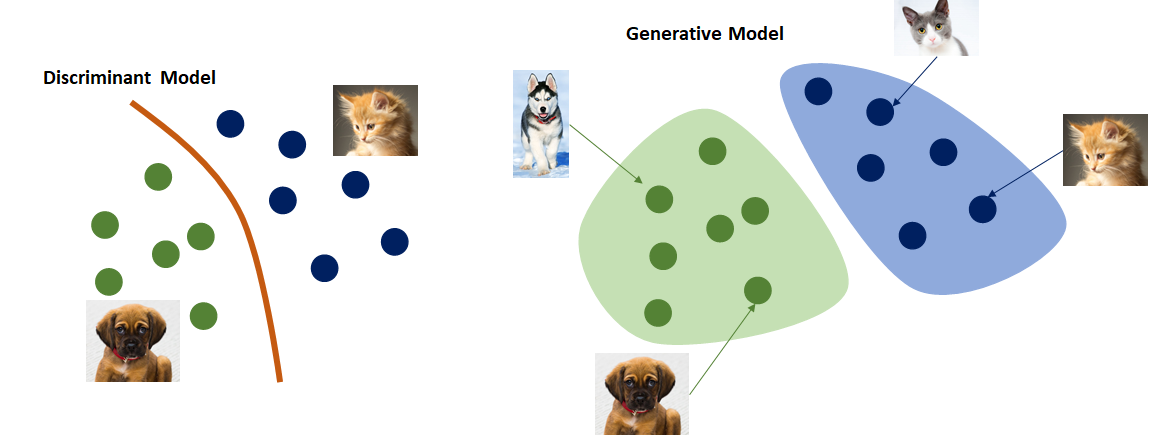
\includegraphics[width=10cm]{gen_disc}
			      \caption{Discriminative vs Generative Models \href{https://medium.com/@jordi299/about-generative-and-discriminative-models-d8958b67ad32}{Source}}
		      \end{figure}

	\end{itemize}
}


\frame{\frametitle{Generative Models}

	\begin{itemize}
		\item Generative models have two types:
		      \begin{itemize}
			      \item \alert{Explicit likelihood models} are defined by an explicit specification of the density, and so their unnormalized complete likelihood can be usually expressed in closed form.
			      \item \alert{Implicit probabilistic models} are defined naturally in a sampling procedure and often induce a likelihood function that cannot be expressed explicitly.
		      \end{itemize}
	\end{itemize}
	\begin{figure}
		\centering
		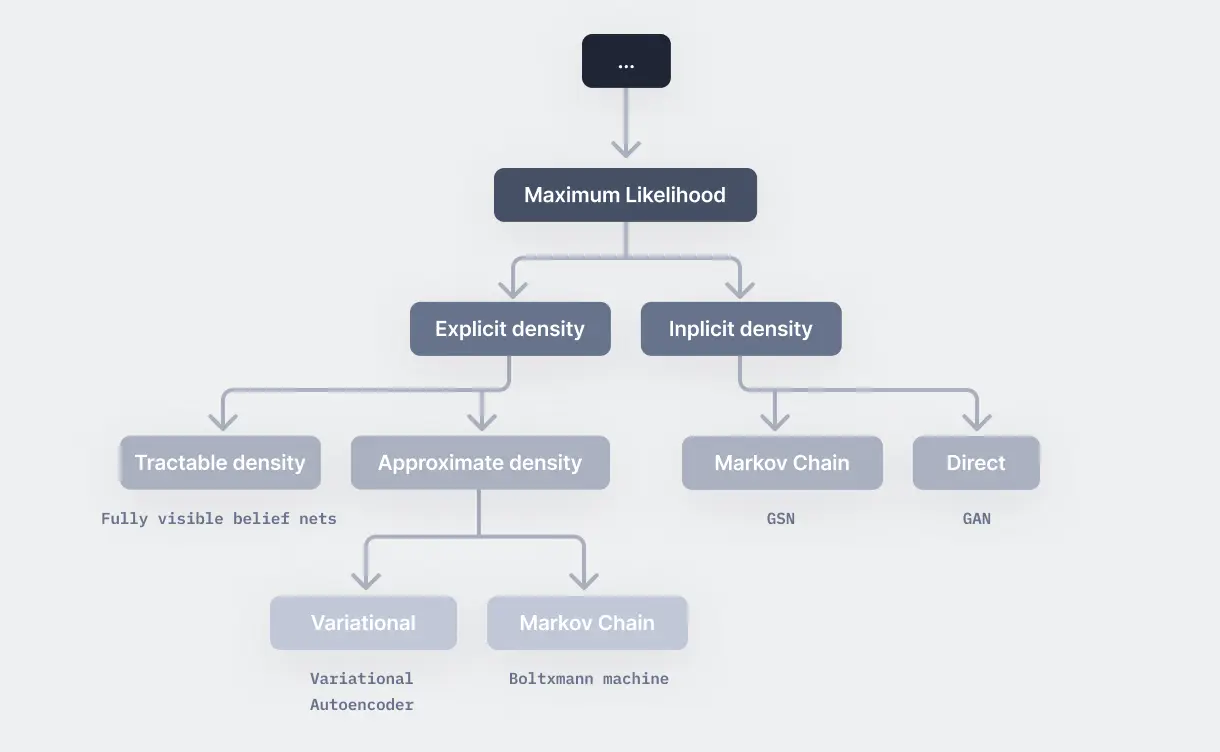
\includegraphics[width=6cm]{gen_models}
		\caption{IAN Goodfellow's presentation of Generative Models Taxonomy \href{https://arxiv.org/pdf/1701.00160.pdf}{Source}}
	\end{figure}
}

\frame{\frametitle{Generative Models}
	\begin{itemize}
		\item Generative models aim for a complete probabilistic description of the data. With these models, the goal is to construct the joint probability distribution $P(X, Y)$ – either directly or by first computing $P(X | Y)$ and $P(Y)$ – and then inferring the conditional probabilities required to classify new data.
		\item Generative models are used for:
		      \begin{enumerate}
			      \item \alert{Density estimation} is the task of estimating the probability density function (PDF) of a random variable.
			      \item \alert{Data generation} is the task of generating new data samples from a given distribution.
			      \item \alert{Data imputation} is the task of filling in missing data.
			      \item \alert{Data compression} is the task of reducing the amount of information required to represent a dataset.
		      \end{enumerate}
	\end{itemize}
}
\section{Architecture}

\frame{\frametitle{Generative Adversarial Networks - Architecture}
	\begin{itemize}
		\item So how do Generative Adversarial Networks work?
		\item GAN composes of two deep networks:
		      \begin{itemize}
			      \item The generator
			      \item The discriminator.
		      \end{itemize}
	\end{itemize}

	\hyperlink{gan}{
		\begin{figure}
			\centering
			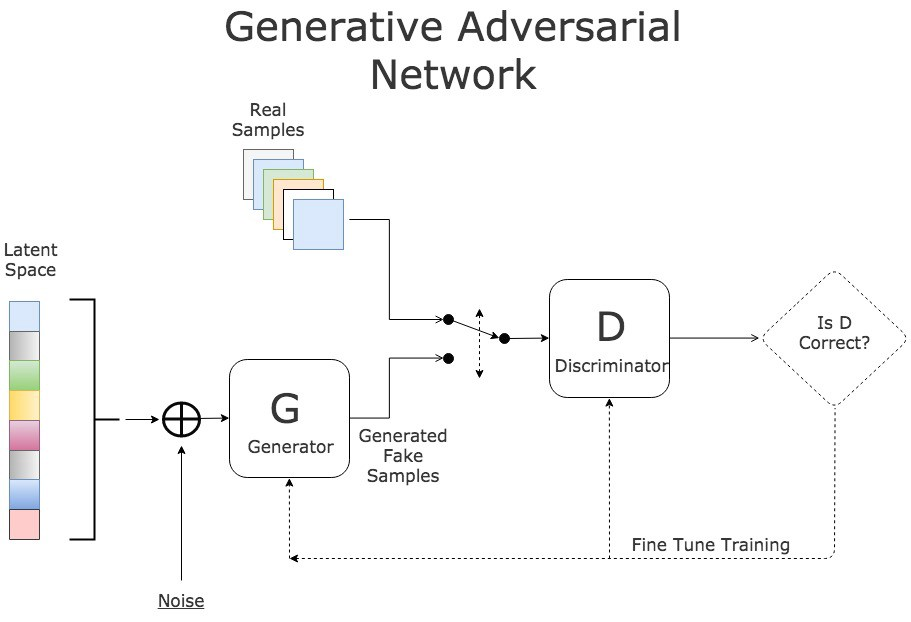
\includegraphics[width=7cm]{gan.jpeg}
		\end{figure}
	}
}

\frame{\frametitle{Generative Adversarial Networks - Structure}
	\hyperlink{gan_structure}{
		\begin{figure}
			\centering
			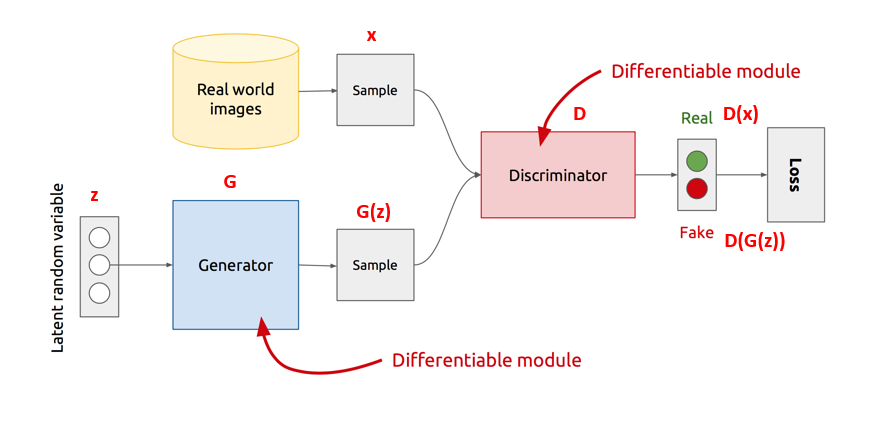
\includegraphics[width=6cm]{../images/GAN_Structure.png}
		\end{figure}
	}

	\begin{itemize}
		\item So let's look at the full picture
		\item Let $G_\phi$ be the generator and $D_\theta$ be the discriminator ($\phi$ and $\theta$ are the parameters of $G$ and $D$, respectively)
		\item We have a neural network based generator which takes as input a noise vector $z \sim N(0, I)$ and produces $G_\phi(z) = X$
		\item We have a neural network based discriminator which could take as input a real $X$ or a generated $X = G_\phi(z)$ and classify the input as real/fake
	\end{itemize}
}


\frame{\frametitle{GAN: Loss Function}
	\begin{center}
		\tikzstyle{hidden_neuron}=[circle,draw=blue!50,fill=cyan!10,thick,minimum size=4mm]
\begin{tikzpicture}
\newcommand*{\xpos}{10}
\newcommand*{\ypos}{10}
\newcommand*{\rectstarty}{6}
\newcommand*{\rectendy}{6.5}


%%%%%%%%%%%%%%Generator

% Generator
{
	\renewcommand*{\xpos}{20}
	\draw[rounded corners,fill=green!12] (\xpos-0.5, \rectstarty+1) rectangle (\xpos+2, \rectendy+1) {};
	\node (N) at (\xpos+0.75,\rectendy+0.75) {\small{Generator}};

	% Sample z
	\draw[rounded corners,fill=cyan!20] (\xpos-0.5, \rectstarty) rectangle (\xpos+2, \rectendy) {};
	\node[hidden_neuron] (N1) at (\xpos,\rectstarty+0.25) {};
	\node[hidden_neuron] (N2) at (\xpos+1*0.5,\rectstarty+0.25) {};
	\node[hidden_neuron] (N3) at (\xpos+2*0.5,\rectstarty+0.25) {};
	\node[hidden_neuron] (N4) at (\xpos+3*0.5,\rectstarty+0.25) {};
	\node (N) at (\xpos+1,\rectstarty-0.5) {\small{$z \sim N(0,I)$}};

	% Bottom arrow
	\draw[->,thick,black] (\xpos+0.75,\rectendy) -- (\xpos+0.75,\rectendy+0.5);

	% Images
	\node (N) at (\xpos+0.75,\rectstarty+2.2) {
\includegraphics[scale=0.1]{images/two_gen.png}};

	% Top arrow
	\draw[->,thick,black] (\xpos+0.75,\rectendy+1) -- (\xpos+0.75,\rectendy+1.5);
}
%%%%%%%%%%%%%%%Real world images
{
	\renewcommand*{\xpos}{23}

	% Real Images
	\draw[rounded corners,fill=green!12] (\xpos-0.5, \rectstarty+1) rectangle (\xpos+2, \rectendy+1) {};
	\node (N) at (\xpos+0.75,\rectendy+0.75) {\small{Real Images}};

	% Images
	\node (N) at (\xpos+0.75,\rectstarty+2.2) {
\includegraphics[scale=0.1]{images/two_real.png}};

	% Top arrow
	\draw[->,thick,black] (\xpos+0.75,\rectendy+1) -- (\xpos+0.75,\rectendy+1.5);

	\renewcommand*{\xpos}{23}
	\draw[->,thick,black] (\xpos+0.75,\rectendy+1.9) -- (\xpos+0.75-0.7,\rectstarty+3);
}
%%%%%%%%%%%%%%%% Discriminator
{
	\renewcommand*{\xpos}{21.5}
	% Discriminator
	\draw[rounded corners,fill=green!12] (\xpos-0.5, \rectstarty+3) rectangle (\xpos+2, \rectendy+3) {};
	\node (N) at (\xpos+0.75,\rectendy+2.75) {\small{Discriminator	}};
	{
		\draw[->,thick,black] (\xpos+0.75,\rectendy+3) -- (\xpos+0.75,\rectendy+3.4);
		\node (N) at (\xpos+0.75,\rectendy+3.52) {\small {Real or Fake}};
	}

	% Arrows
	\renewcommand*{\xpos}{20}
	\draw[->,thick,black] (\xpos+0.75,\rectendy+1.9) -- (\xpos+0.75+0.7,\rectstarty+3);
}
\end{tikzpicture}
	\end{center}

	\begin{itemize}
		\item What should be the objective function of the overall network?
		\item Let's look at the objective function of the generator first
		\item Given an image generated by the generator as $G_\phi(z)$ the discriminator assigns a score $D_\theta(G_\phi(z))$ to it
		\item This score will be between $0$ and $1$ and will tell us the probability of the image being real or fake
	\end{itemize}
}

\frame{\frametitle{GAN: Loss Function}
	\vspace*{-1cm}
	\begin{itemize}
		\item For a given $z$, the generator would want to maximize  $\log D_\theta(G_\phi(z))$ (log likelihood) or minimize $\log (1 - D_\theta(G_\phi(z)))$
		\item This is just for a single $z$ and the generator would like to do this for all possible values of $z$,
		\item For example, if $z$ was discrete and drawn from a uniform distribution (\textit{i.e.}, $p(z) = \frac{1}{N} ~ \forall z$) then the generator's objective function would be
		      $$ \min\limits_{\phi}  \sum_{i=1}^{N} \frac{1}{N} \log (1 - D_{\theta}(G_{\phi}(z))) $$
	\end{itemize}
}

\frame{\frametitle{GAN: Loss Function}
	\begin{itemize}
		\item However, in our case, z is continuous and not uniform ($z \sim N(0, I)$) so the equivalent objective function would be
		      $$\min \limits_{\phi} \int p(z) \log(1 - D_{\theta}(G_{\phi}(z)))$$
		      $$\min \limits_{\phi}  E_{_{z \sim p(z)}} [\log (1 - D_{\theta}(G_{\phi}(z)))] $$
	\end{itemize}

	\hyperlink{Binglin}{
		\begin{figure}
			\centering
			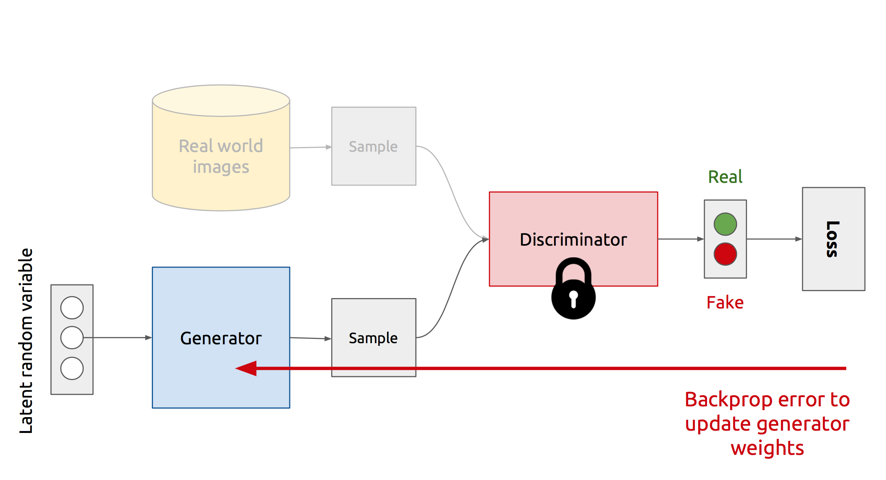
\includegraphics[width=8cm]{../images/Gen.png}
		\end{figure}
	}
}

\frame{\frametitle{GAN: Loss Function}
	\hyperlink{Binglin}{
		\begin{figure}
			\centering
			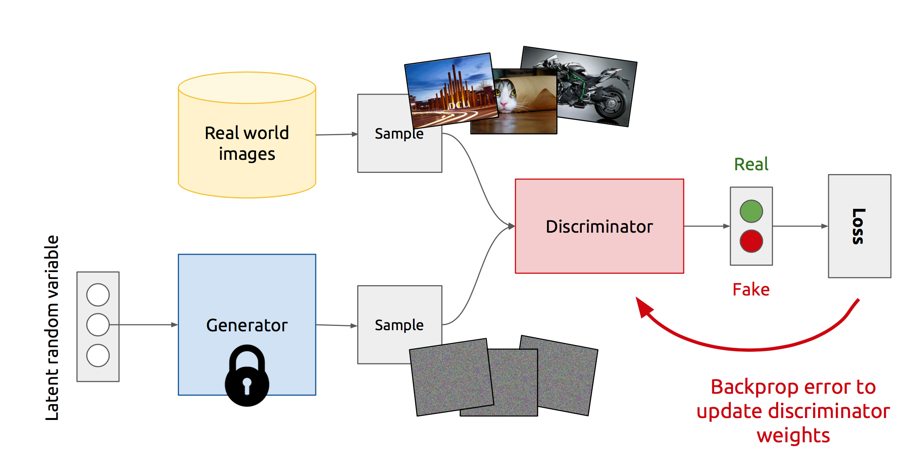
\includegraphics[width=8cm]{../images/Disc.png}
		\end{figure}
	}
	\begin{itemize}
		\item Now let's look at the discriminator
		\item The task of the discriminator is to assign a high score to real images and a low score to fake images
		\item And it should do this for all possible real images and all possible fake images
		\item In other words, it should try to maximize the following objective function
		      $$ \max_{\theta} E_{_{x \sim p_{data}}} [\log D_{\theta}(x)]
			      \newline + E_{_{z \sim p(z)}} [\log (1 - D_{\theta}(G_{\phi}(z)))] $$
	\end{itemize}
}

\frame{\frametitle{GAN: Loss Function}
	\vspace*{-1cm}
	\begin{itemize}
		\item If we put the objectives of the generator and discriminator together we get a minimax game
		      \begin{align*}
			      \min\limits_{\phi}\hspace*{2mm} \max\limits_{\theta} \hspace*{4mm} [ & \mathbb{E}_{x \sim p_{data}} \log D_{\theta}(x)                   \\
			                                                                           & ~~~+ \mathbb{E}_{z \sim p(z)} \log(1- D_{\theta}(G_{\phi}(z)) ) ]
		      \end{align*}
		\item The first term in the objective is only w.r.t. the parameters of the discriminator ($\theta$)

		\item The second term in the objective is w.r.t. the parameters of the generator ($\phi$) as well as the discriminator ($\theta$)
		\item The discriminator wants to maximize the second term whereas the generator wants to minimize it (hence it is a two-player game)
	\end{itemize}
}
\section{Training}

\begin{frame}
	\frametitle{GAN - Training}
	\begin{itemize}
		\item So the overall training proceeds by alternating between these two step

		\item \textbf{Step 1:} Gradient Ascent on Discriminator
		      $$ \max\limits_{\theta}\hspace*{2mm} [\mathbb{E}_{x \sim p_{data}} \log D_{\theta}(x)
			      \newline
			      + \mathbb{E}_{z \sim p(z)} \log(1- D_{\theta}(G_{\phi}(z)) ) ]$$

		\item \textbf{Step 2:} Gradient Descent on Generator
		      $$   \min\limits_{\phi}\hspace*{2mm} \mathbb{E}_{z \sim p(z)} \log(1- D_{\theta}(G_{\phi}(z)) )$$

		\item In practice, the above generator objective does not work well and we use a slightly modified objective
		\item Let us see why
	\end{itemize}
\end{frame}

\frame{\frametitle{GAN - Training}
	\begin{center}
		\hyperlink{miteshk}{
			\begin{figure}
				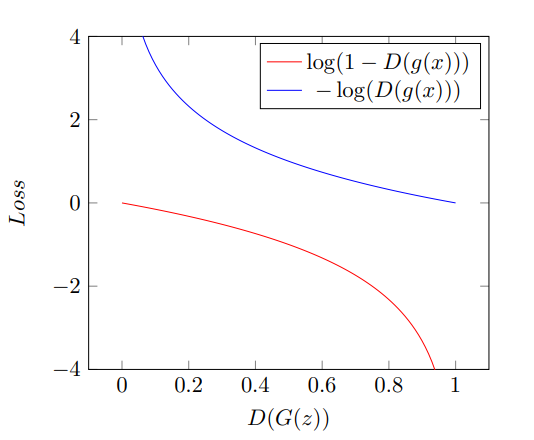
\includegraphics[width=5cm]{images/chart.png}
			\end{figure}
		}
	\end{center}
	\begin{itemize}
		\item When the sample is likely fake, we want to give a feedback to the generator (using gradients)
		\item However, in this region where $D(G(z))$ is close to 0, the curve of the loss function is very flat and the gradient would be close to $0$
		\item Trick: Instead of minimizing the likelihood of the discriminator being correct, maximize the likelihood of the discriminator being wrong
		\item In effect, the objective remains the same but the gradient signal becomes better
	\end{itemize}
}
